\documentclass[]{article}


%-----------------------------------------------------------------------------------------------------------------------------------------
%
%   GLOBALS
%
%-----------------------------------------------------------------------------------------------------------------------------------------
\newcommand{\DOCTITLE}{

}
\newcommand{\DOCAUTHOR}{

}
\newcommand{\DISCLAIMER}
{
    \topskip0pt
    \vspace*{\fill}
    {
    \centering
        \small{
            THIS DOCUMENT IS INTENDED FOR INTERNAL USE ONLY
        }
    }
    \\
    {
    \centering
        \small{
        UNAUTHORIZED DISTRIBUTION OF THIS DOCUMENT IS STRICTLY PROHIBITED 
        }
    }
    \vspace*{\fill}
}

\usepackage{lmodern}
\usepackage{amssymb,amsmath}
\usepackage{ifxetex,ifluatex}
\usepackage{fixltx2e} % provides \textsubscript
\ifnum 0\ifxetex 1\fi\ifluatex 1\fi=0 % if pdftex
  \usepackage[T1]{fontenc}
  \usepackage[utf8]{inputenc}
\else % if luatex or xelatex
  \ifxetex
    \usepackage{mathspec}
    \usepackage{xltxtra,xunicode}
  \else
    \usepackage{fontspec}
  \fi
  \defaultfontfeatures{Mapping=tex-text,Scale=MatchLowercase}
  \newcommand{\euro}{€}
\fi
% use upquote if available, for straight quotes in verbatim environments
\IfFileExists{upquote.sty}{\usepackage{upquote}}{}
% use microtype if available
\IfFileExists{microtype.sty}{%
\usepackage{microtype}
\UseMicrotypeSet[protrusion]{basicmath} % disable protrusion for tt fonts
}{}
\ifxetex
  \usepackage[setpagesize=false, % page size defined by xetex
              unicode=false, % unicode breaks when used with xetex
              xetex]{hyperref}
\else
  \usepackage[unicode=true]{hyperref}
\fi
\usepackage[usenames,dvipsnames]{color}
\hypersetup{breaklinks=true,
            bookmarks=true,
            pdfauthor={},
            pdftitle={},
            colorlinks=true,
            citecolor=blue,
            urlcolor=blue,
            linkcolor=magenta,
            pdfborder={0 0 0}}
\urlstyle{same}  % don't use monospace font for urls
\usepackage{graphicx,grffile}
\makeatletter
\def\maxwidth{\ifdim\Gin@nat@width>\linewidth\linewidth\else\Gin@nat@width\fi}
\def\maxheight{\ifdim\Gin@nat@height>\textheight\textheight\else\Gin@nat@height\fi}
\makeatother
% Scale images if necessary, so that they will not overflow the page
% margins by default, and it is still possible to overwrite the defaults
% using explicit options in \includegraphics[width, height, ...]{}
\setkeys{Gin}{width=\maxwidth,height=\maxheight,keepaspectratio}
\setlength{\parindent}{0pt}
\setlength{\parskip}{6pt plus 2pt minus 1pt}
\setlength{\emergencystretch}{3em}  % prevent overfull lines
\providecommand{\tightlist}{%
  \setlength{\itemsep}{0pt}\setlength{\parskip}{0pt}}
\setcounter{secnumdepth}{0}

\date{}

% Redefines (sub)paragraphs to behave more like sections
\ifx\paragraph\undefined\else
\let\oldparagraph\paragraph
\renewcommand{\paragraph}[1]{\oldparagraph{#1}\mbox{}}
\fi
\ifx\subparagraph\undefined\else
\let\oldsubparagraph\subparagraph
\renewcommand{\subparagraph}[1]{\oldsubparagraph{#1}\mbox{}}
\fi

%-----------------------------------------------------------------------------------------------------------------------------------------
%
%   PAGE SIZE AND MARGINS
%
%-----------------------------------------------------------------------------------------------------------------------------------------
\usepackage[a4paper,headheight=30pt]{geometry}
%\usepackage[letterpaper, portrait, margin=2in]{geometry}
\addtolength{\topmargin}{-.5in}
\addtolength{\textheight}{1.75in}

\usepackage{graphicx}

\usepackage{fancyhdr}
\pagestyle{fancy}


%-----------------------------------------------------------------------------------------------------------------------------------------
% Page break after sections
%-----------------------------------------------------------------------------------------------------------------------------------------
%\usepackage{titlesec}
%\newcommand{\sectionbreak}{\clearpage}

\lhead{
    %left header content
%    \topskip0pt
%    \vspace*{\fill}
    {
    \centering
        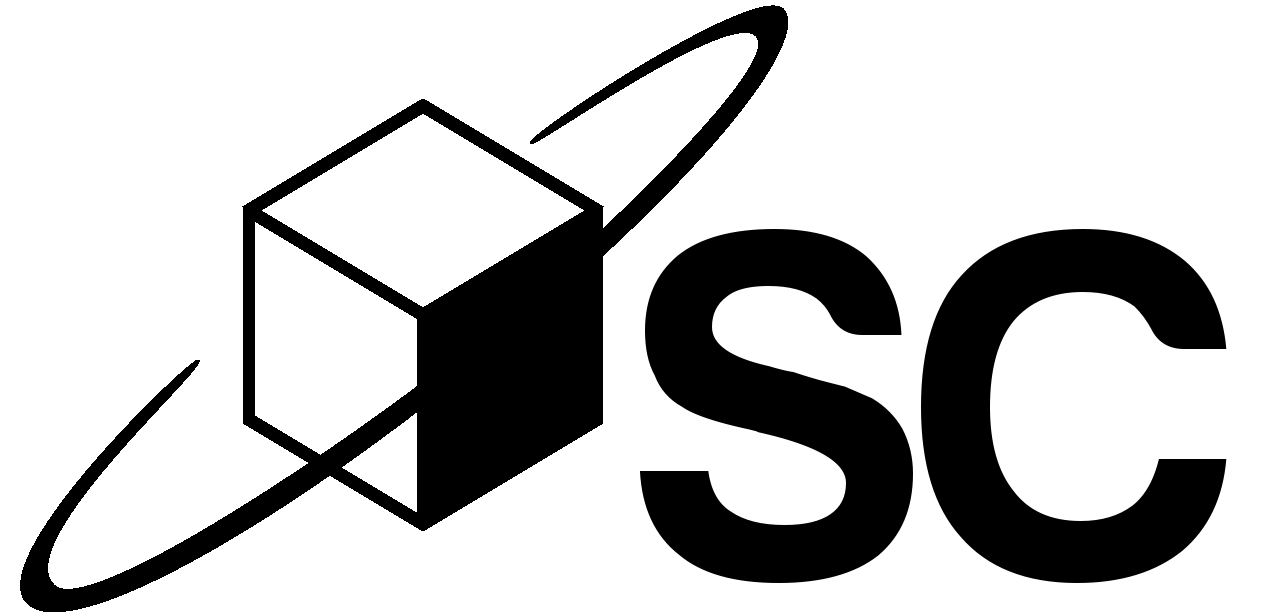
\includegraphics[height=2.66em]{template/sc.png}
    }
%    \vspace*{\fill}
}
\chead{
    \topskip0pt
    \vspace*{\fill}
    {
    \centering
        \small{
            THIS DOCUMENT IS INTENDED FOR INTERNAL USE ONLY
        }
    }
    \\
    {
    \centering
        \small{
        UNAUTHORIZED DISTRIBUTION OF THIS DOCUMENT IS STRICTLY PROHIBITED 
        }
    }
    \vspace*{\fill}
}
\rhead{
%    \topskip0pt
%    \vspace*{\fill}
    % right header content
    {
    \centering
        
\includegraphics[height=3.25em]{template/scrd.png}
    }
%    \vspace*{\fill}
}
\lfoot{
    % left footer content
    \topskip0pt
    \vspace*{\fill}
    SCRD
    Revision 0.1
    \vspace*{\fill}
}
\cfoot{
    % middle footer content
    \topskip0pt
    \vspace*{\fill}
    {
    \centering
    SCRD Internal Documents Template \\
    \today
    }
    \vspace*{\fill}
}
\rfoot{
    % right footer content
    \topskip0pt
    \vspace*{\fill}
    \thepage
    \vspace*{\fill}
}
% extend the header into the margins
\usepackage{calc}
\fancyheadoffset[L,R]{\marginparsep+\marginparwidth}

%--------------------------------------------------------------------------------------------------------------
%	My Packages
%--------------------------------------------------------------------------------------------------------------
\usepackage{capt-of}

%--------------------------------------------------------------------------------------------------------------
%
%	BEGIN DOCUMENT
%
%--------------------------------------------------------------------------------------------------------------
\begin{document}


%--------------------------------------------------------------------------------------------------------------
%
%	TITLE PAGE
%
%--------------------------------------------------------------------------------------------------------------
\begin{titlepage}

\newcommand{\HRule}{\rule{\linewidth}{0.5mm}} % Defines a new command for the horizontal lines, change thickness here

\center % Center everything on the page
 
%----------------------------------------------------------------------------------------
%	HEADING SECTIONS
%----------------------------------------------------------------------------------------

\includegraphics[width=200pt,height=200pt]{../images/rocketry_logo_large.png}\\[1cm] % Include a department/university logo - this will require the graphicx package
\textsc{\Large Space Concordia - Rocketry Division}\\[0.5cm] % Major heading such as course name
\textsc{\large Aurelius CR-2-4G - Structural Team}\\[0.5cm] % Minor heading such as course title

%----------------------------------------------------------------------------------------
%	LOGO SECTION
%----------------------------------------------------------------------------------------

\begin{figure}[ht]
    \centering
    \includegraphics[height=100pt]{../images/vertical_model_simplified.png}\\
\end{figure}

%----------------------------------------------------------------------------------------
%	TITLE SECTION
%----------------------------------------------------------------------------------------

\HRule \\[0.6cm]
{ \Huge \bfseries 
Engineering Simulation for Rocket Flight Analysis
}\\[0.4cm] 

\HRule \\[1cm]
 
%----------------------------------------------------------------------------------------
%	AUTHOR SECTION
%----------------------------------------------------------------------------------------

\begin{minipage}{0.4\textwidth}
\begin{flushleft} \large
	\begin{tabular} {r l} 
        \emph{Author(s):} & Shawn Bulger	\\
	\end{tabular}
\end{flushleft}
\end{minipage}
~
\begin{minipage}{0.4\textwidth}
\begin{flushright} \large
	\begin{tabular} {r l} 
		\emph{Coordinator:} & Dr. Ashok Kaushal 		\\
		\emph{Supervisor:}  & Dr. Mehdi Hojjati 		\\
		\emph{EIR:}         & Dominic Ng  		        \\
	\end{tabular}
\end{flushright}
\end{minipage}\\[2cm]

%----------------------------------------------------------------------------------------
%	DATE SECTION
%----------------------------------------------------------------------------------------

{\large \today}\\[2cm] % Date, change the \today to a set date if you want to be precise

\vfill % Fill the rest of the page with whitespace

\end{titlepage}

{
\hypersetup{linkcolor=black}
\setcounter{tocdepth}{3}
\tableofcontents
\clearpage
}
\listoftables
\listoffigures
\clearpage
\section{\texorpdfstring{Vertical (AOA \textless{} 5\(^\circ\)) Flight
Model}{Vertical (AOA \textless{} 5\^{}\textbackslash{}circ) Flight Model}}\label{vertical-aoa-5circ-flight-model}

\subsection{Particular Assumptions}\label{particular-assumptions}

The rocket is to be launched on a guide that may have a \(\pm\)
5\(^\circ\) angle. Considering the small angle approximation, the sine
of 5 degrees or less is approximately equal to the angle in radians, or
zero.

For a 1\% error:

\begin{equation} 
sin ( \theta \le 15^\circ ) \approx 0 
\end{equation}

{[}1{]}

This assumption greatly simplifies the simulation analysis. We consider
that the rocket flies perfectly vertical (experiencing no significant
drift) into still (quiescent) air for which density is described by the
\href{https://en.wikipedia.org/wiki/International_Standard_Atmosphere}{International
Standard Atmosphere (ISA) model}.

\subsection{Simplified Model}\label{simplified-model}

The dynamics of the rocket flights can be simplified to a sum of forces.

Simplifying the rocket flight as ideally one-dimensional, with the
positive z-direction being upwards from the launch pad, the impulse is
equal to the thrust of the rocket minus the weight of the rocket and the
drag forces of the rocket interacting with the surrounding air.

\begin{equation}
\label{eq_vertical_flight_eom}
m(t)\ddot{z}(t) = T(t) - D(\dot{z}) - W(t)
\end{equation}

Mass is a function of time, which is explained in the \emph{Dynamic
Parameters} section. Drag is a function of velocity, which is explained
in \emph{Drag Model} section. Acceleration can be expressed as the first
derivative of velocity and also the second derivative of position, each
with respect to time.

\begin{equation}
\vec{a} = \dot{v} = \ddot{z}
\end{equation}

Each force component can be rearranged and expressed as follows:

\begin{equation}
\vec{a}_T = \dfrac{T(t)}{m(t)}, \vec{a}_W = \dfrac{W(t)}{m(t)}, \vec{a}_D = \dfrac{D(v)}{m(t)}
\end{equation}

The net upward acceleration is: \(\vec{a}_T - \vec{a}_W - \vec{a}_D\)

The sum of forces can be rearranged and acceleration can be solved for:

\begin{equation}
\label{vertical_flight_equation}
\vec{a} =  \ddot{z} = \dfrac{1}{m(t)} (T(t) - D(\dot{z}) - W(t)) 
\end{equation}

Acceleration can be integrated to find position and velocity.

\begin{equation}
\vec{v} = \int \vec{a} dz
\end{equation}

\begin{equation}
z = \iint \vec{a} dz
\end{equation}

Integration of equation (\ref{vertical_flight_equation}) in the model is
represented by the \(\dfrac{1}{s}\) block. The model is pictured in
Figure \ref{vertical_model_simplified}.

\begin{figure}[htbp]
\centering
\includegraphics{images/vertical_model_simplified.png}
\caption{Vertical Flight Model - Simplified
\label{vertical_model_simplified}}
\end{figure}

\subsection{Drift due to
Weathercocking}\label{drift-due-to-weathercocking}

\emph{Weathercocking} is a phenomenon when the rocket tends to alter its
trajectory and fly into the wind. If the rocket is stable, and has a
sufficiently high damping ratio, the rocket eventually reaches a
near-zero angle-of-attack parallel to the velocity vector of the wind,
only in the opposite direction.

We can modify Equation \ref{eq_vertical_flight_eom} to account for
weathercocking and provide the actual altitude reached, as well as the
amount of drift experienced.

Altitude accounting for weathercocking

\begin{equation}
\label{eq_vertical_angle}
m(t)_z\ddot{z}(t) = T(t) \cos \theta - D(\dot{z}) \cos \theta - W(t)
\end{equation}

Where:

\begin{itemize}
\tightlist
\item
  \(z\) is the upward direction (normal from the ground)
\item
  \(\theta\) is the angle between the current rocket trajectory and the
  z-axis
\end{itemize}

Drift accounting for weathercocking

\begin{equation}
\label{eq_vertical_angle}
m(t)_x \ddot{z}(t) = T(t) \sin \theta - D(\dot{z}) \sin \theta 
\end{equation}

\hyperdef{}{refs}{\label{refs}}
\hyperdef{}{ref-optics2004}{\label{ref-optics2004}}
{[}1{]} ``Intro optics pPT v1part 04.pdf.'' Online.

\end{document}
